\documentclass{stdlocal}
\begin{document}
\begin{minipage}[b]{\textwidth}
  \center
  \begin{minipage}[b]{0.4\textwidth}
    \center
    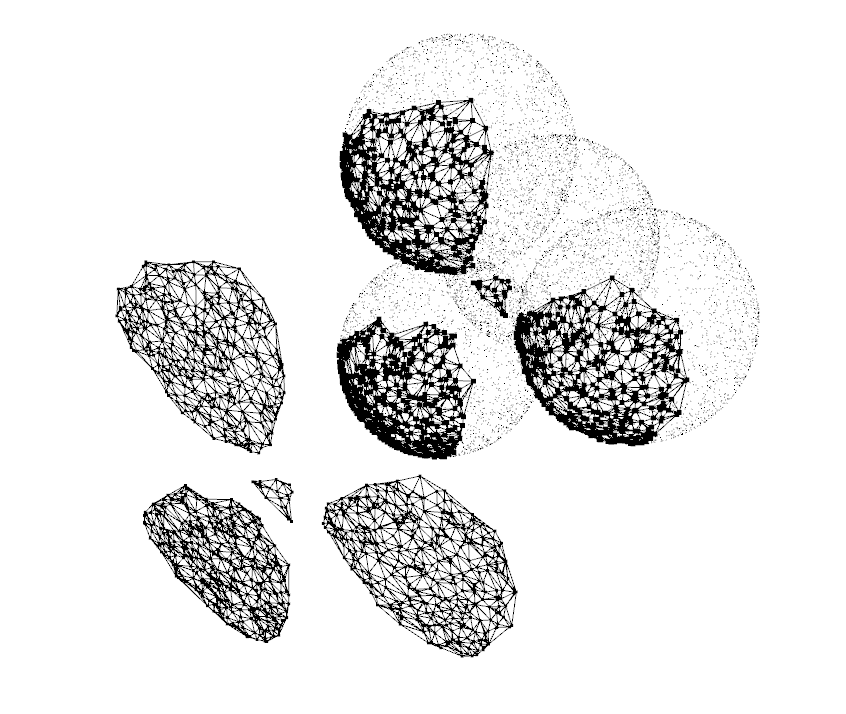
\includegraphics[width=0.8\textwidth]{../../images/3d_pareto_front_tessellation_01.png}
  \end{minipage}
  \begin{minipage}[b]{0.4\textwidth}
    \center
    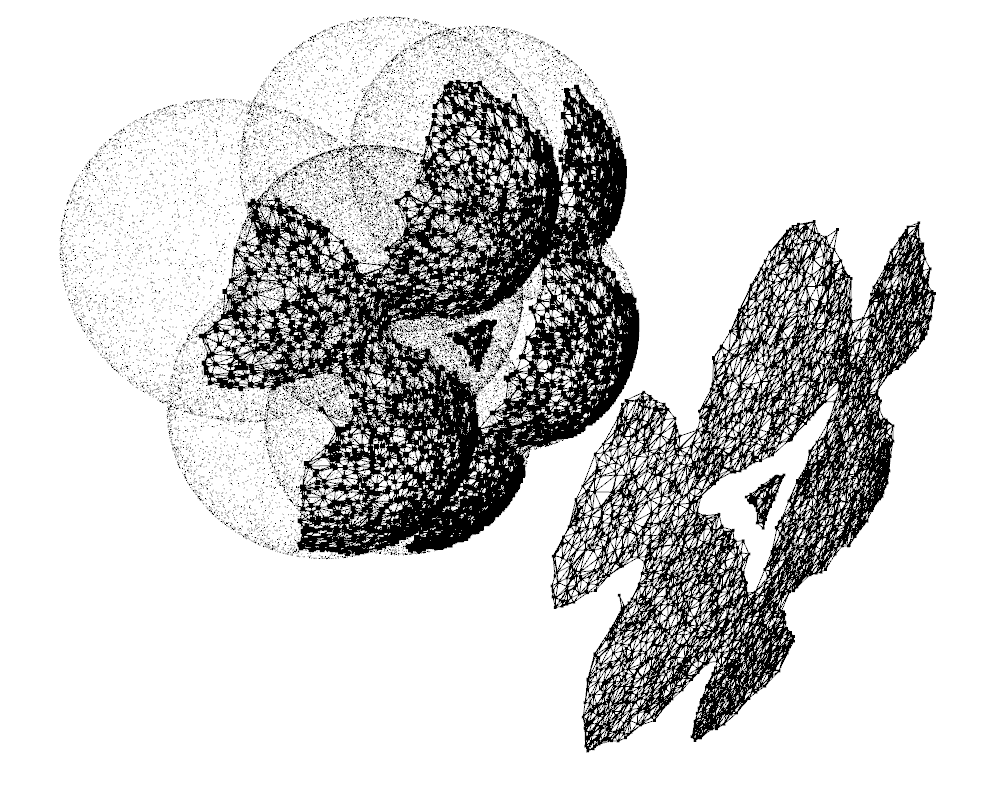
\includegraphics[width=0.8\textwidth]{../../images/3d_pareto_front_tessellation_02.png}
  \end{minipage}
\end{minipage}
\bigskip
\hrule
\smallskip
% \begin{abstract}
  \begin{center}
    \textbf{Abstract}
  \end{center}
  \itshape
  \hspace{10pt}
  Multiobjective optimization plays a key role in computer-aided design, manufacturing, and engineering.
  Typical problems need to find a trade-off between many conflicting objectives.
  Because no single solution exists, human intervention is necessary to provide a preference and choose between different Pareto-optimal solutions.
  In real-world applications, this possibility should be given by a configuration interface.
  But in general, solving a multiobjective problem only involves estimating a set of unsorted and nondominated points near the actual Pareto frontier.
  Hence, a configuration interface for humans, used to choose one of those optimal solutions, is not able to proper visualize solutions or to offer an intuitive user interface.
  This paper explores the possibility of tessellating $n$-dimensional Pareto frontiers based on projection, Delaunay triangulation, and a statistical heuristic to generate a hypersurface and make visualization and configuration feasible.
  The developed algorithm has been tested against standard, constructed, and real test problems.
% \end{abstract}
\bigskip
\hrule
\bigskip
\end{document}